\documentclass[twoside]{book}

% Packages required by doxygen
\usepackage{fixltx2e}
\usepackage{calc}
\usepackage{doxygen}
\usepackage[export]{adjustbox} % also loads graphicx
\usepackage{graphicx}
\usepackage[utf8]{inputenc}
\usepackage{makeidx}
\usepackage{multicol}
\usepackage{multirow}
\PassOptionsToPackage{warn}{textcomp}
\usepackage{textcomp}
\usepackage[nointegrals]{wasysym}
\usepackage[table]{xcolor}

% Font selection
\usepackage[T1]{fontenc}
\usepackage[scaled=.90]{helvet}
\usepackage{courier}
\usepackage{amssymb}
\usepackage{sectsty}
\renewcommand{\familydefault}{\sfdefault}
\allsectionsfont{%
  \fontseries{bc}\selectfont%
  \color{darkgray}%
}
\renewcommand{\DoxyLabelFont}{%
  \fontseries{bc}\selectfont%
  \color{darkgray}%
}
\newcommand{\+}{\discretionary{\mbox{\scriptsize$\hookleftarrow$}}{}{}}

% Page & text layout
\usepackage{geometry}
\geometry{%
  a4paper,%
  top=2.5cm,%
  bottom=2.5cm,%
  left=2.5cm,%
  right=2.5cm%
}
\tolerance=750
\hfuzz=15pt
\hbadness=750
\setlength{\emergencystretch}{15pt}
\setlength{\parindent}{0cm}
\setlength{\parskip}{3ex plus 2ex minus 2ex}
\makeatletter
\renewcommand{\paragraph}{%
  \@startsection{paragraph}{4}{0ex}{-1.0ex}{1.0ex}{%
    \normalfont\normalsize\bfseries\SS@parafont%
  }%
}
\renewcommand{\subparagraph}{%
  \@startsection{subparagraph}{5}{0ex}{-1.0ex}{1.0ex}{%
    \normalfont\normalsize\bfseries\SS@subparafont%
  }%
}
\makeatother

% Headers & footers
\usepackage{fancyhdr}
\pagestyle{fancyplain}
\fancyhead[LE]{\fancyplain{}{\bfseries\thepage}}
\fancyhead[CE]{\fancyplain{}{}}
\fancyhead[RE]{\fancyplain{}{\bfseries\leftmark}}
\fancyhead[LO]{\fancyplain{}{\bfseries\rightmark}}
\fancyhead[CO]{\fancyplain{}{}}
\fancyhead[RO]{\fancyplain{}{\bfseries\thepage}}
\fancyfoot[LE]{\fancyplain{}{}}
\fancyfoot[CE]{\fancyplain{}{}}
\fancyfoot[RE]{\fancyplain{}{\bfseries\scriptsize Generated by Doxygen }}
\fancyfoot[LO]{\fancyplain{}{\bfseries\scriptsize Generated by Doxygen }}
\fancyfoot[CO]{\fancyplain{}{}}
\fancyfoot[RO]{\fancyplain{}{}}
\renewcommand{\footrulewidth}{0.4pt}
\renewcommand{\chaptermark}[1]{%
  \markboth{#1}{}%
}
\renewcommand{\sectionmark}[1]{%
  \markright{\thesection\ #1}%
}

% Indices & bibliography
\usepackage{natbib}
\usepackage[titles]{tocloft}
\setcounter{tocdepth}{3}
\setcounter{secnumdepth}{5}
\makeindex

% Custom commands
\newcommand{\clearemptydoublepage}{%
  \newpage{\pagestyle{empty}\cleardoublepage}%
}

\usepackage{caption}
\captionsetup{labelsep=space,justification=centering,font={bf},singlelinecheck=off,skip=4pt,position=top}

%===== C O N T E N T S =====

\begin{document}

% Titlepage & ToC
\pagenumbering{roman}
\begin{titlepage}
\vspace*{7cm}
\begin{center}%
{\Large My Project }\\
\vspace*{1cm}
{\large Generated by Doxygen 1.8.11}\\
\end{center}
\end{titlepage}
\clearemptydoublepage
\tableofcontents
\clearemptydoublepage
\pagenumbering{arabic}

%--- Begin generated contents ---
\chapter{Hierarchical Index}
\section{Class Hierarchy}
This inheritance list is sorted roughly, but not completely, alphabetically\+:\begin{DoxyCompactList}
\item \contentsline{section}{Numerical\+Solver}{\pageref{class_numerical_solver}}{}
\item \contentsline{section}{pub\+Sub\+Helper}{\pageref{structpub_sub_helper}}{}
\item \contentsline{section}{Sensor}{\pageref{class_sensor}}{}
\begin{DoxyCompactList}
\item \contentsline{section}{G\+PS}{\pageref{class_g_p_s}}{}
\item \contentsline{section}{I\+MU}{\pageref{class_i_m_u}}{}
\item \contentsline{section}{M\+RU}{\pageref{class_m_r_u}}{}
\item \contentsline{section}{Speed\+Sensor}{\pageref{class_speed_sensor}}{}
\end{DoxyCompactList}
\item \contentsline{section}{Vessel}{\pageref{class_vessel}}{}
\item \contentsline{section}{Vessel\+Node}{\pageref{class_vessel_node}}{}
\item \contentsline{section}{Weather}{\pageref{class_weather}}{}
\end{DoxyCompactList}

\chapter{Class Index}
\section{Class List}
Here are the classes, structs, unions and interfaces with brief descriptions\+:\begin{DoxyCompactList}
\item\contentsline{section}{{\bf G\+PS} }{\pageref{class_g_p_s}}{}
\item\contentsline{section}{{\bf I\+MU} }{\pageref{class_i_m_u}}{}
\item\contentsline{section}{{\bf M\+RU} }{\pageref{class_m_r_u}}{}
\item\contentsline{section}{{\bf Numerical\+Solver} }{\pageref{class_numerical_solver}}{}
\item\contentsline{section}{{\bf pub\+Sub\+Helper} }{\pageref{structpub_sub_helper}}{}
\item\contentsline{section}{{\bf Sensor} }{\pageref{class_sensor}}{}
\item\contentsline{section}{{\bf Speed\+Sensor} }{\pageref{class_speed_sensor}}{}
\item\contentsline{section}{{\bf Vessel} }{\pageref{class_vessel}}{}
\item\contentsline{section}{{\bf Vessel\+Node} }{\pageref{class_vessel_node}}{}
\item\contentsline{section}{{\bf Weather} }{\pageref{class_weather}}{}
\end{DoxyCompactList}

\chapter{Class Documentation}
\section{G\+PS Class Reference}
\label{class_g_p_s}\index{G\+PS@{G\+PS}}
Inheritance diagram for G\+PS\+:\begin{figure}[H]
\begin{center}
\leavevmode
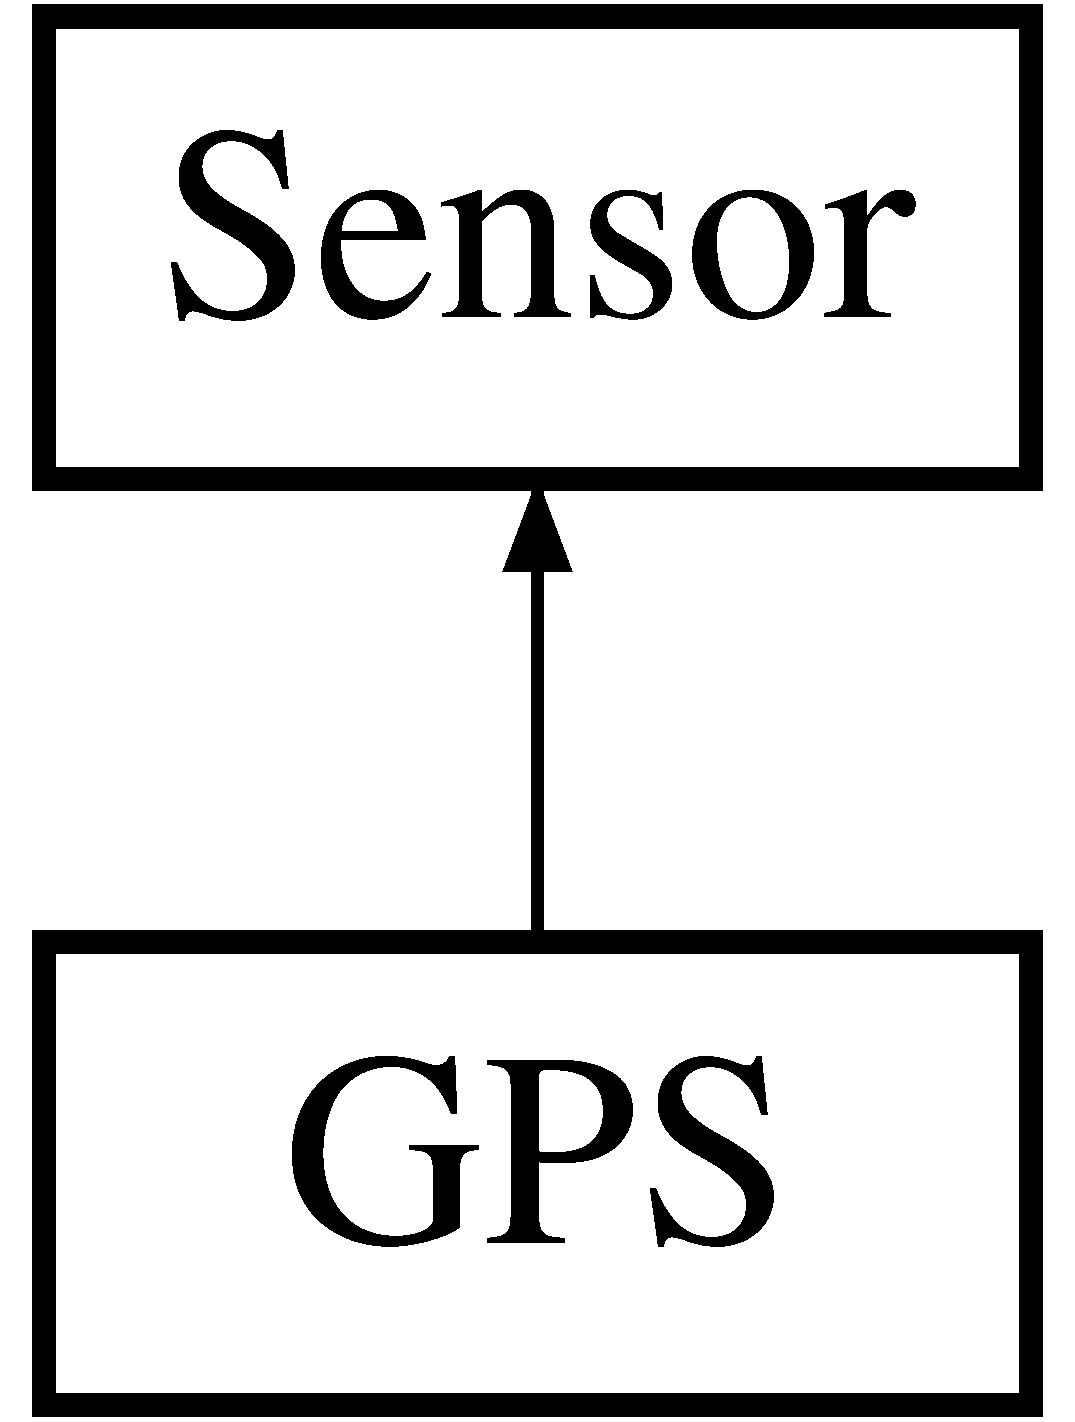
\includegraphics[height=2.000000cm]{class_g_p_s}
\end{center}
\end{figure}
\subsection*{Public Member Functions}
\begin{DoxyCompactItemize}
\item 
void {\bfseries receive\+Start\+Coordinates} (double latitute\+\_\+start, double longitude\+\_\+start)\label{class_g_p_s_a0d42ac91be4e0f9c53735f60029dac69}

\item 
void {\bfseries publish\+Gps\+Data} (Vector6d nu\+\_\+n, Vector6d eta)\label{class_g_p_s_a772b3562596d25e2992f21c923f29d32}

\end{DoxyCompactItemize}
\subsection*{Additional Inherited Members}


The documentation for this class was generated from the following files\+:\begin{DoxyCompactItemize}
\item 
include/gps.\+h\item 
src/gps.\+cpp\end{DoxyCompactItemize}

\section{I\+MU Class Reference}
\label{class_i_m_u}\index{I\+MU@{I\+MU}}
Inheritance diagram for I\+MU\+:\begin{figure}[H]
\begin{center}
\leavevmode
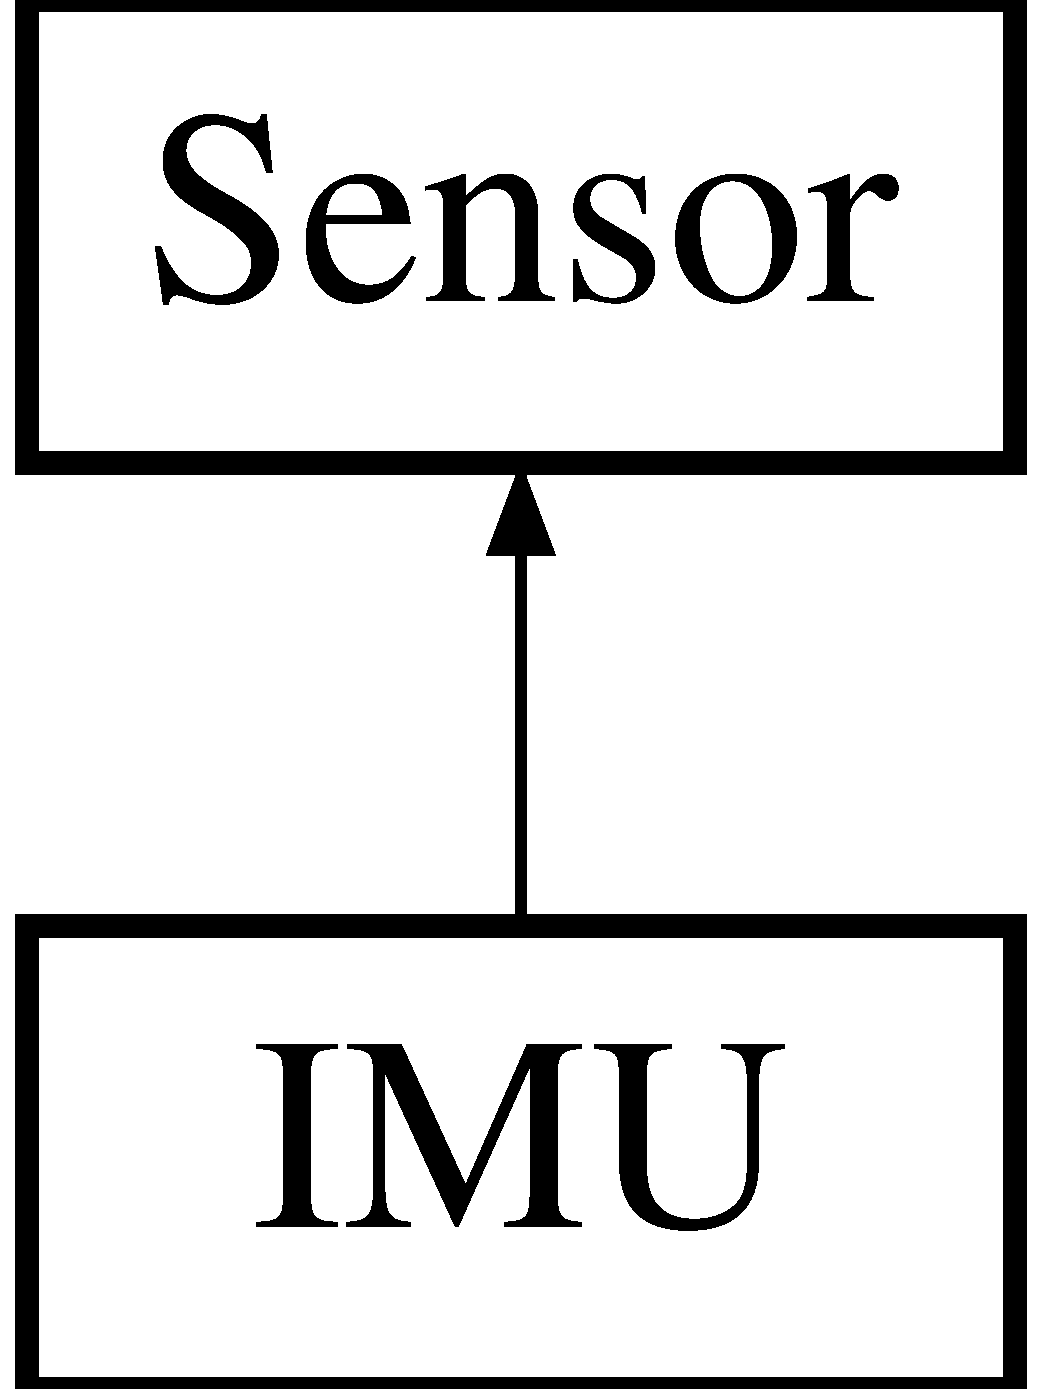
\includegraphics[height=2.000000cm]{class_i_m_u}
\end{center}
\end{figure}
\subsection*{Public Member Functions}
\begin{DoxyCompactItemize}
\item 
void {\bfseries publish\+Imu\+Data} (Vector6d nu\+\_\+dot, Vector6d nu)\label{class_i_m_u_a2d525fcbec09c226ec4c7df75f52a623}

\end{DoxyCompactItemize}
\subsection*{Additional Inherited Members}


The documentation for this class was generated from the following files\+:\begin{DoxyCompactItemize}
\item 
include/imu.\+h\item 
src/imu.\+cpp\end{DoxyCompactItemize}

\section{M\+RU Class Reference}
\label{class_m_r_u}\index{M\+RU@{M\+RU}}
Inheritance diagram for M\+RU\+:\begin{figure}[H]
\begin{center}
\leavevmode
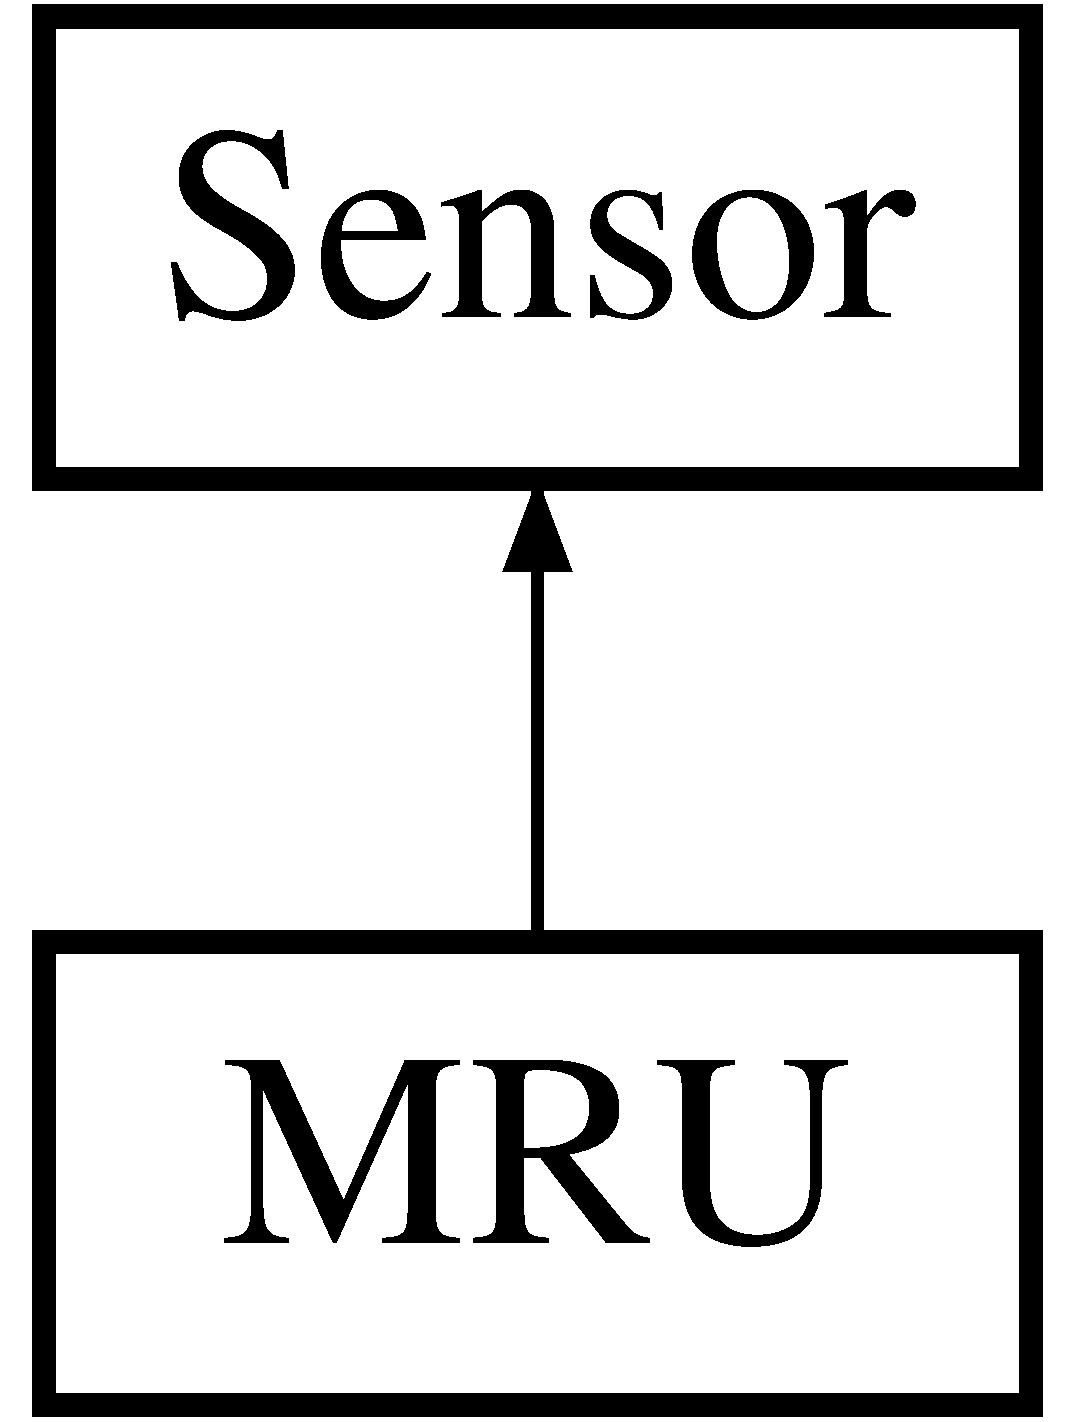
\includegraphics[height=2.000000cm]{class_m_r_u}
\end{center}
\end{figure}
\subsection*{Public Member Functions}
\begin{DoxyCompactItemize}
\item 
void {\bfseries publish\+Mru\+Data} (Vector6d nu, Vector6d eta)\label{class_m_r_u_ac3926b4ce79a4ddc075597bf8a20114e}

\end{DoxyCompactItemize}
\subsection*{Additional Inherited Members}


The documentation for this class was generated from the following files\+:\begin{DoxyCompactItemize}
\item 
include/mru.\+h\item 
src/mru.\+cpp\end{DoxyCompactItemize}

\section{Numerical\+Solver Class Reference}
\label{class_numerical_solver}\index{Numerical\+Solver@{Numerical\+Solver}}
\subsection*{Public Member Functions}
\begin{DoxyCompactItemize}
\item 
void {\bfseries initialize\+Solver} (double dt)\label{class_numerical_solver_ac91717b927990eae2c14f01b4f5d14bc}

\end{DoxyCompactItemize}
\subsection*{Public Attributes}
\begin{DoxyCompactItemize}
\item 
long double {\bfseries epsilon}\label{class_numerical_solver_afb8890c4e2ca28d83618ebb8d5d92a40}

\item 
long double {\bfseries t}\label{class_numerical_solver_a820f9ececb6053b7c698b713fe63b8d4}

\item 
long double {\bfseries y}\label{class_numerical_solver_abfd49621bc1dc6a3d9ab17fcf927e900}

\item 
long double {\bfseries h}\label{class_numerical_solver_a61c3dbeb72ea9e38497cab19e2a13dd0}

\item 
long double {\bfseries h\+\_\+min}\label{class_numerical_solver_ae084d982a43c4e79dfc64709a98bf2a8}

\item 
long double {\bfseries h\+\_\+max}\label{class_numerical_solver_acf5b7cda252abcad36fc7cd4744d94ee}

\item 
long double {\bfseries a21}\label{class_numerical_solver_a4a12d3cb2fe4d57959c4afadf83587fe}

\item 
long double {\bfseries a31}\label{class_numerical_solver_ac7342c2cc07fe0615c67c0201f18b6f2}

\item 
long double {\bfseries a32}\label{class_numerical_solver_aab4f92c00be318b92ddb98490b74873c}

\item 
long double {\bfseries a41}\label{class_numerical_solver_a03392893e3f74427a1a9e37e95b68d38}

\item 
long double {\bfseries a42}\label{class_numerical_solver_a5296cbd0ddb9831e9956c449a4e6cd8f}

\item 
long double {\bfseries a43}\label{class_numerical_solver_a7e4b18d68e7dcde10516f8235a0d7f30}

\item 
long double {\bfseries a51}\label{class_numerical_solver_a83fea8ee882c5ce66bab8cc1e9e8dbc8}

\item 
long double {\bfseries a52}\label{class_numerical_solver_ae3c12d6b4663e9e440b85aee47c8b47b}

\item 
long double {\bfseries a53}\label{class_numerical_solver_a88bf012d7679849890b0b1972051ec88}

\item 
long double {\bfseries a54}\label{class_numerical_solver_a958f7b76784d340ac947179bd7c24b81}

\item 
long double {\bfseries a61}\label{class_numerical_solver_ae071af6e19e60053b854d2cd8db5c652}

\item 
long double {\bfseries a62}\label{class_numerical_solver_a430fe6458279b591395e75076744d7cb}

\item 
long double {\bfseries a63}\label{class_numerical_solver_ae6b9e8d173b12139cda750ec391b040d}

\item 
long double {\bfseries a64}\label{class_numerical_solver_a106096496b16b7766d6df4648ebeba5e}

\item 
long double {\bfseries a65}\label{class_numerical_solver_a68f838e70f4e9a48572361fed9be0d37}

\item 
long double {\bfseries a71}\label{class_numerical_solver_a3a317078414074b35576a56b52c990e9}

\item 
long double {\bfseries a72}\label{class_numerical_solver_a7e39ec51fe853923df65ae2beea5c052}

\item 
long double {\bfseries a73}\label{class_numerical_solver_a9f95c14fab884bf26aa28925dd11fafb}

\item 
long double {\bfseries a74}\label{class_numerical_solver_aaf7b397e5d20e9d231f41815b7d449df}

\item 
long double {\bfseries a75}\label{class_numerical_solver_a5a9ea766c579b905b2db2b13a2515bab}

\item 
long double {\bfseries a76}\label{class_numerical_solver_a6f8184a3b4c2617889cc09b9c23f55e2}

\item 
long double {\bfseries c2}\label{class_numerical_solver_a4eb3e49b7a0b1fdd22563418fcabfd77}

\item 
long double {\bfseries c3}\label{class_numerical_solver_a0570fa7009b46ce177caef91a3c5e1cf}

\item 
long double {\bfseries c4}\label{class_numerical_solver_a625be6001aa5e1dd7d36ad66c3d7f9ff}

\item 
long double {\bfseries c5}\label{class_numerical_solver_a4f9fef3a4e2996b63d064c2833195aa7}

\item 
long double {\bfseries c6}\label{class_numerical_solver_ac1f0a84f237acbafbdc03b81c0f8c775}

\item 
long double {\bfseries c7}\label{class_numerical_solver_ada4bd22795caa2a04083bf4d329be842}

\item 
long double {\bfseries b11}\label{class_numerical_solver_ad8e9b376edb4947c43a63fff1febac30}

\item 
long double {\bfseries b12}\label{class_numerical_solver_ade1238dee1b62e9e2592889ac06048c0}

\item 
long double {\bfseries b13}\label{class_numerical_solver_ae69c75b1d7ecd2f62dc29f23230ba1af}

\item 
long double {\bfseries b14}\label{class_numerical_solver_a092eae02f3835e4612090373e66f6264}

\item 
long double {\bfseries b15}\label{class_numerical_solver_a6e1da4c2d5ea3efd65fdc60b85d4fe6e}

\item 
long double {\bfseries b16}\label{class_numerical_solver_a6756b4ba3befd89e1f1e21eeaecc0d11}

\item 
long double {\bfseries b17}\label{class_numerical_solver_a0e8605020eeaa4c804cfba14e3579e0b}

\item 
long double {\bfseries b21}\label{class_numerical_solver_a98f579fad728d51b64ed620aba39119e}

\item 
long double {\bfseries b22}\label{class_numerical_solver_a9d0fd5b94af289c06400b6b1a0faae93}

\item 
long double {\bfseries b23}\label{class_numerical_solver_a24def4410d7104761f697b6cff8fc057}

\item 
long double {\bfseries b24}\label{class_numerical_solver_adcadb6d5073426e00cee9009642e2bf9}

\item 
long double {\bfseries b25}\label{class_numerical_solver_a7e189696b82f961428aace50a8de16fa}

\item 
long double {\bfseries b26}\label{class_numerical_solver_a353b1e5d87fff5b4a21dcb99fcaff04d}

\item 
long double {\bfseries b27}\label{class_numerical_solver_a9e239affbdac0b6072d6b44243b708d4}

\item 
Vector6d {\bfseries k1v}\label{class_numerical_solver_a93ef81dfb4ef831a5450bf8fa837a9a7}

\item 
Vector6d {\bfseries k2v}\label{class_numerical_solver_acc393c1ef473672544099ad982899440}

\item 
Vector6d {\bfseries k3v}\label{class_numerical_solver_a9d591f1d328805ec3126cb1c06b9cf24}

\item 
Vector6d {\bfseries k4v}\label{class_numerical_solver_a5008982363bc64e6470d3f2b21f2fe5e}

\item 
Vector6d {\bfseries k5v}\label{class_numerical_solver_a20b7c5b49cf40832eebc0758e9dda731}

\item 
Vector6d {\bfseries k6v}\label{class_numerical_solver_a1472bad71e92d0c36e181784841af4dd}

\item 
Vector6d {\bfseries k7v}\label{class_numerical_solver_a346e784e7ed2a87f86d7d9742ad9e28a}

\item 
Vector6d {\bfseries zv}\label{class_numerical_solver_a91c473d6e9a890cfaff1ffd8252d6647}

\item 
Vector6d {\bfseries sv}\label{class_numerical_solver_a77191b6497e19b1c979faf7ae6577408}

\item 
Vector6d {\bfseries errv}\label{class_numerical_solver_a1e67e7d370ffcbda9f00f62b67f2b222}

\end{DoxyCompactItemize}


The documentation for this class was generated from the following files\+:\begin{DoxyCompactItemize}
\item 
include/solver.\+h\item 
src/solver.\+cpp\end{DoxyCompactItemize}

\section{pub\+Sub\+Helper Struct Reference}
\label{structpub_sub_helper}\index{pub\+Sub\+Helper@{pub\+Sub\+Helper}}
\subsection*{Public Member Functions}
\begin{DoxyCompactItemize}
\item 
void {\bfseries callback} (const geometry\+\_\+msgs\+::\+Twist\+::\+Const\+Ptr \&msg)\label{structpub_sub_helper_ad078027647718453f1340be7d43332e8}

\end{DoxyCompactItemize}
\subsection*{Public Attributes}
\begin{DoxyCompactItemize}
\item 
int {\bfseries num\+Rec\+Messages} = 0\label{structpub_sub_helper_a9ff07f43c4df37706418b77548236461}

\end{DoxyCompactItemize}


The documentation for this struct was generated from the following file\+:\begin{DoxyCompactItemize}
\item 
src/unittest.\+cpp\end{DoxyCompactItemize}

\section{Sensor Class Reference}
\label{class_sensor}\index{Sensor@{Sensor}}
Inheritance diagram for Sensor\+:\begin{figure}[H]
\begin{center}
\leavevmode
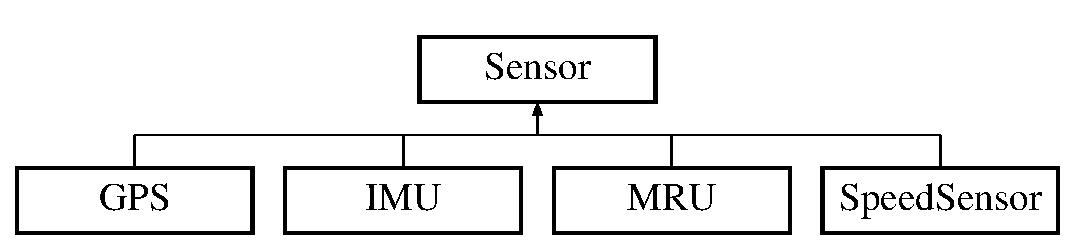
\includegraphics[height=2.000000cm]{class_sensor}
\end{center}
\end{figure}
\subsection*{Public Member Functions}
\begin{DoxyCompactItemize}
\item 
void {\bfseries publish\+Data} (Vector6d v\+\_\+n, Vector3d gps\+\_\+info)\label{class_sensor_a45ddf880a759f03d22818e91860f0901}

\item 
void {\bfseries publish\+Data} (double u, double v)\label{class_sensor_a7fc20251253ec330e00725cf00688ee0}

\item 
void {\bfseries publish\+Data} (Vector6d imu\+\_\+data)\label{class_sensor_a5f103439ae3ed1cb84e8a35705a3c032}

\item 
void {\bfseries publish\+Data} (Vector6d nu, Vector6d eta)\label{class_sensor_af44389030d7336c5a24a87588bb31448}

\item 
void {\bfseries set\+Step\+Size} (double stepsize)\label{class_sensor_ae37c1cfa48a7f25497aae485f6f91265}

\item 
void {\bfseries set\+Frequency} (double \+\_\+frequency)\label{class_sensor_afe6b7b2849deccb1818da714de6c36ad}

\item 
void {\bfseries set\+Noise} ()\label{class_sensor_ac4b9625c973636b3f3c574bc7b2a922d}

\end{DoxyCompactItemize}
\subsection*{Public Attributes}
\begin{DoxyCompactItemize}
\item 
ros\+::\+Node\+Handle {\bfseries sensor\+\_\+handle}\label{class_sensor_a3b3c9b96c4ed4ff563181b74fc518b5c}

\item 
ros\+::\+Publisher {\bfseries gps\+\_\+pub} = sensor\+\_\+handle.\+advertise$<$simulator\+\_\+prototype\+::\+Gps$>$(\char`\"{}sensors/gps\char`\"{}, 0)\label{class_sensor_a811e9071506ad8925dba54b9e40ab5a2}

\item 
ros\+::\+Publisher {\bfseries mru\+\_\+velocity\+\_\+pub} = sensor\+\_\+handle.\+advertise$<$geometry\+\_\+msgs\+::\+Twist$>$(\char`\"{}sensors/mru/velocity\char`\"{}, 0)\label{class_sensor_a56727fc8fe63502e44d365297b5666ea}

\item 
ros\+::\+Publisher {\bfseries mru\+\_\+position\+\_\+pub} = sensor\+\_\+handle.\+advertise$<$geometry\+\_\+msgs\+::\+Twist$>$(\char`\"{}sensors/mru/position\char`\"{}, 0)\label{class_sensor_a08cb49aa8df3a84c5bb5546b1c11323e}

\item 
ros\+::\+Publisher {\bfseries imu\+\_\+pub} = sensor\+\_\+handle.\+advertise$<$geometry\+\_\+msgs\+::\+Twist$>$(\char`\"{}sensors/imu\char`\"{}, 0)\label{class_sensor_ab2f14e6d6c5a19338689e7af04fff45e}

\item 
ros\+::\+Publisher {\bfseries speed\+\_\+sensor\+\_\+pub} = sensor\+\_\+handle.\+advertise$<$geometry\+\_\+msgs\+::\+Twist$>$(\char`\"{}sensors/speed\+Sensor\char`\"{}, 0)\label{class_sensor_afc9a4388ae0a7d8bec357af261e9c4a8}

\item 
double {\bfseries dt}\label{class_sensor_ae6f4e03bbd96a9c020ee0b737c23a7bf}

\item 
double {\bfseries frequency}\label{class_sensor_a9cc770795c32650dc738d52e900c7c37}

\item 
double {\bfseries steps\+\_\+per\+\_\+data\+\_\+output}\label{class_sensor_a3409fcd46e7ba87534325b78b40a93d2}

\item 
double {\bfseries step}\label{class_sensor_a2a9811c9f9fc04523f98276fdc794219}

\end{DoxyCompactItemize}


The documentation for this class was generated from the following files\+:\begin{DoxyCompactItemize}
\item 
include/sensor.\+h\item 
src/sensor.\+cpp\end{DoxyCompactItemize}

\section{Speed\+Sensor Class Reference}
\label{class_speed_sensor}\index{Speed\+Sensor@{Speed\+Sensor}}
Inheritance diagram for Speed\+Sensor\+:\begin{figure}[H]
\begin{center}
\leavevmode
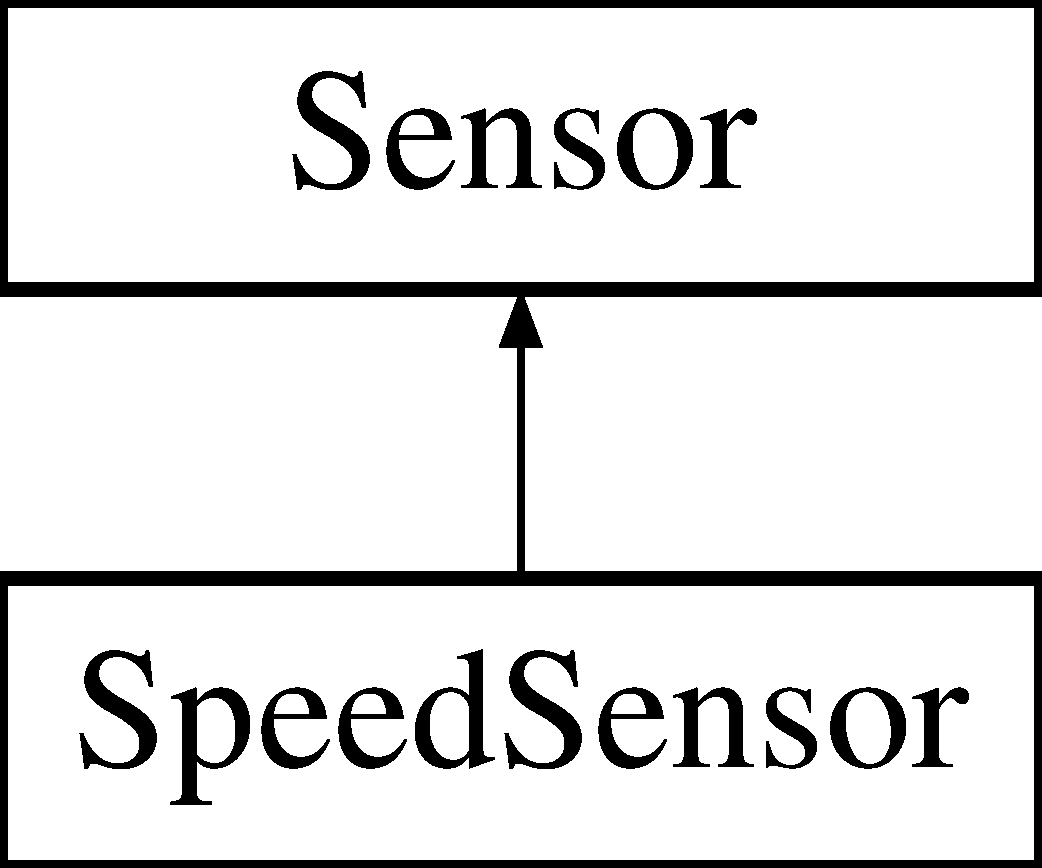
\includegraphics[height=2.000000cm]{class_speed_sensor}
\end{center}
\end{figure}
\subsection*{Public Member Functions}
\begin{DoxyCompactItemize}
\item 
void {\bfseries publish\+Speed\+Sensor\+Data} (double u, double v)\label{class_speed_sensor_ae141c26517458aac01a12281a7f6b96f}

\end{DoxyCompactItemize}
\subsection*{Additional Inherited Members}


The documentation for this class was generated from the following files\+:\begin{DoxyCompactItemize}
\item 
include/speedsensor.\+h\item 
src/speedsensor.\+cpp\end{DoxyCompactItemize}

\section{Vessel Class Reference}
\label{class_vessel}\index{Vessel@{Vessel}}
\subsection*{Public Member Functions}
\begin{DoxyCompactItemize}
\item 
Vector6d {\bfseries get\+Thrust} ()\label{class_vessel_a2ce81e44b7ee78b485fca9fc36e66a80}

\item 
void {\bfseries set\+Thrust} (Vector6d tau\+\_\+in)\label{class_vessel_a5249717b95a643331fede0213ed53d0c}

\item 
bool {\bfseries read\+Parameters} (ros\+::\+Node\+Handle nh)\label{class_vessel_aad41e1742883df3fa8fb6e2f42e49c8e}

\item 
void {\bfseries initialize\+Matrices} ()\label{class_vessel_ac9b3616a8650590abc6f73ce24d840ee}

\item 
void {\bfseries initialize\+State\+Vectors} ()\label{class_vessel_a3cc8cc98ec3d1b3fab2f675047501447}

\item 
void {\bfseries initialize\+Sensors} ()\label{class_vessel_ad8b014067732ad92dc9912884afbd0e9}

\item 
void {\bfseries step} ()\label{class_vessel_a26bd848c65e8697f89106ead6632f512}

\item 
double {\bfseries get\+DT} ()\label{class_vessel_a3f29ece8a16cda2896d7774083ea7f52}

\item 
void {\bfseries set\+State} (Vector6d eta, Vector6d nu)\label{class_vessel_ac57b48a077ff7e815b589ab734c10b05}

\item 
void {\bfseries get\+State} (Vector6d \&eta, Vector6d \&nu)\label{class_vessel_a7946e31d788a7d18ca5b398982c2b29e}

\end{DoxyCompactItemize}
\subsection*{Public Attributes}
\begin{DoxyCompactItemize}
\item 
double {\bfseries M\+\_\+det}\label{class_vessel_a6a8f75c5777179900640c93dc1691a25}

\end{DoxyCompactItemize}


The documentation for this class was generated from the following files\+:\begin{DoxyCompactItemize}
\item 
include/vessel.\+h\item 
src/vessel.\+cpp\end{DoxyCompactItemize}

\section{Vessel\+Node Class Reference}
\label{class_vessel_node}\index{Vessel\+Node@{Vessel\+Node}}
\subsection*{Public Member Functions}
\begin{DoxyCompactItemize}
\item 
void {\bfseries step} ()\label{class_vessel_node_a3441573289fe061665c8d4b32a9445c7}

\item 
double {\bfseries get\+DT} ()\label{class_vessel_node_a471b1ea921f3baccc95ffb7a0b7f6db3}

\end{DoxyCompactItemize}
\subsection*{Public Attributes}
\begin{DoxyCompactItemize}
\item 
{\bf Vessel} {\bfseries vessel}\label{class_vessel_node_a2096cf24b7129b8011be9e0b101e6e7c}

\end{DoxyCompactItemize}


The documentation for this class was generated from the following files\+:\begin{DoxyCompactItemize}
\item 
include/vesselnode.\+h\item 
src/vesselnode.\+cpp\end{DoxyCompactItemize}

\section{Weather Class Reference}
\label{class_weather}\index{Weather@{Weather}}
\subsection*{Public Member Functions}
\begin{DoxyCompactItemize}
\item 
void {\bfseries Set\+Wind\+Data} (double mean\+\_\+wind\+\_\+speed\+\_\+in, double mean\+\_\+wind\+\_\+angle\+\_\+in, double height)\label{class_weather_a48d1098ede2e0cf3fc61102cb551bc5e}

\item 
void {\bfseries Set\+Current\+Data} (double mean\+\_\+current\+\_\+speed\+\_\+in, double mean\+\_\+current\+\_\+angle\+\_\+in)\label{class_weather_a4b2bc213fef6bf759426f783a0a91aec}

\end{DoxyCompactItemize}
\subsection*{Public Attributes}
\begin{DoxyCompactItemize}
\item 
double {\bfseries wind\+\_\+angle}\label{class_weather_acc253d38bec71dddfb4ae92af380c6e5}

\item 
double {\bfseries current\+\_\+angle}\label{class_weather_ab304533a7f025f1a2f3c112038255110}

\item 
double {\bfseries wind\+\_\+speed}\label{class_weather_a3bf8124bffb9977bb431cca94a9dcc6e}

\item 
double {\bfseries current\+\_\+speed}\label{class_weather_a850d28701912b9ab5c38dbe25ceb4374}

\item 
double {\bfseries wind\+\_\+mean\+\_\+speed}\label{class_weather_a16c656d234ae82390ae3d6b0b2c3d25f}

\item 
double {\bfseries wind\+\_\+mean\+\_\+angle}\label{class_weather_a9ba4efa510c11bd8d9ea841a8f59597e}

\item 
double {\bfseries current\+\_\+mean\+\_\+speed}\label{class_weather_ae7433f63d352a8716e954553090b0b03}

\item 
double {\bfseries current\+\_\+mean\+\_\+angle}\label{class_weather_a9df9824cd69668a46db8ee9c15e9d843}

\item 
double {\bfseries wind\+\_\+std\+\_\+dev}\label{class_weather_a42a7e1a8cd76e584e40b9e8f40ba5fb2}

\item 
double {\bfseries current\+\_\+std\+\_\+dev}\label{class_weather_ad10c40b130367299a700e43c716ba991}

\end{DoxyCompactItemize}


The documentation for this class was generated from the following files\+:\begin{DoxyCompactItemize}
\item 
include/weather.\+h\item 
src/weather.\+cpp\end{DoxyCompactItemize}

%--- End generated contents ---

% Index
\backmatter
\newpage
\phantomsection
\clearemptydoublepage
\addcontentsline{toc}{chapter}{Index}
\printindex

\end{document}
